% ---
% type: Article
% title: LaTeX Reference Project
% authors:
%   - type: Person
%     givenNames:
%       - Karl
%       - R
%     familyNames: Popper
%     affiliation:
%       type: University
%       name: University of Canterbury
%       address:
%         type: PostalAddress
%         addressCountry: New Zealand
%         addressLocality: Christchurch
%   - type: Person
%     givenNames: Auguste
%     familyNames: Comte
%     affiliation:
%       - type: Organization
%         name: University of Montpellier
%         url: www.umontpellier.fr/en
%         address:
%           type: PostalAddress
%           addressCountry: France
%           addressLocality: Montpellier
%       - type: Organization
%         name: École Polytechnique      
%         address:
%           type: PostalAddress
%           addressCountry: France
%           addressLocality: Paris
%   - type: Person
%     givenNames: Francis
%     familyNames: Bacon
%     affiliation:
%       - type: Organization
%        name: Trinity College
%        address:
%          type: PostalAddress
%          addressCountry: United Kingdom
%          addressLocality: Cambridge
%        parentOrganization:
%          type: Organization
%          name: University of Cambridge
% bibliography: refs.bib
% ---



\documentclass[12pt]{article}

% --- Packages --- %

\usepackage{authblk} % for marking up authorship; \affil{} command (and customizations)
\usepackage{hyperref} % for hyperlinks; \href{} command
\usepackage{setspace} % for line spacing; \onehalfspacing command
\usepackage{graphicx}
\usepackage{listings}
\usepackage{minted}

% --- Customization --- %

\renewcommand\Affilfont{\fontsize{10}{11}\itshape} % font size of affil

% remove * from thanks
\makeatletter
\def\thanks#1{\protected@xdef\@thanks{\@thanks
        \protect\footnotetext{#1}}}
\makeatother


    
% --- Content --- %

\begin{document}

\onehalfspacing

\title{LaTeX Reference Project}

\author[1]{Karl R. Popper\textsuperscript{*}\thanks{*Authors contributed equally to this study; karl@poppermail.com, comte@astuteauguste.com}}
\author[2,3]{Auguste Comte\textsuperscript{*}}
\author[4]{Francis Bacon}

\affil[1]{University of Canterbury, Christchurch, New Zealand}
\affil[2]{University of Montpellier, Montpellier, France}
\affil[3]{\'{E}cole Polytechnique, Paris, France}
\affil[4]{Trinity College, University of Cambridge, Cambridge, United Kingdom}

\maketitle

\begin{abstract}
In the abstract you will summarize the motivation, results and
conclusions of the manuscript.
The abstract is the most read section of the entire paper, so 
making it concise, precise and punchy is critical.
Sometimes authors write in the present tense, sometimes in the past
tense -- it is more a matter of style.

\end{abstract}

\clearpage

\section*{Introduction}

The present document is meant to help you set up a \LaTeX
(\texttt{.tex}) manuscript to be converted into any format supported by
Stencila.
It has been written by a scientist for scientists; of course, not
everything you can do with \LaTeX  will have found its way into this
tutorial.
If you \textbf{really} need support for some obscure \LaTeX
functionality that Stencila does not already cover, you can make a
pull request (PR) on one of our repositories, like Encoda's
(\href{Encoda repo}{https://stenci.la/encoda}).

\subsection*{YAML commented block at the top}
The attentive reader will have noticed that at the top of this
\texttt{.tex} file, there are many commented lines with \texttt{\%}
containing YAML code:

{\singlespace
\begin{minted}[gobble=0,frame=single,linenos]{yaml}
type: Article
title: LaTeX Reference Project
authors:
  - type: Person
    givenNames:
      - Karl
      - R
    familyNames: Popper
    affiliation:
      type: University
      name: University of Canterbury
      address:
        type: PostalAddress
        addressCountry: New Zealand
        addressLocality: Christchurch
  - type: Person
    givenNames: Auguste
    familyNames: Comte
    affiliation:
      - type: Organization
        name: University of Montpellier
        url: www.umontpellier.fr/en
        address:
          type: PostalAddress
          addressCountry: France
          addressLocality: Montpellier
      - type: Organization
        name: École Polytechnique      
        address:
          type: PostalAddress
          addressCountry: France
          addressLocality: Paris
  - type: Person
    givenNames: Francis
    familyNames: Bacon
    affiliation:
      - type: Organization
       name: Trinity College
       address:
         type: PostalAddress
         addressCountry: United Kingdom
         addressLocality: Cambridge
       parentOrganization:
         type: Organization
         name: University of Cambridge
\end{minted}
}

\noindent (The box above was rendered with the \LaTeX 's \texttt{minted}
package.)

This commented YAML block needs to be at the top of the file so that
Stencila's internal programs can first parse and then reformat the
article's metadata.

\subsection*{Figures}

It is easy to place different kinds of figures.
You can, for example, decorate your manuscript with a photo of the
best animal out there: the panda bear.

\begin{figure}
  \centering
  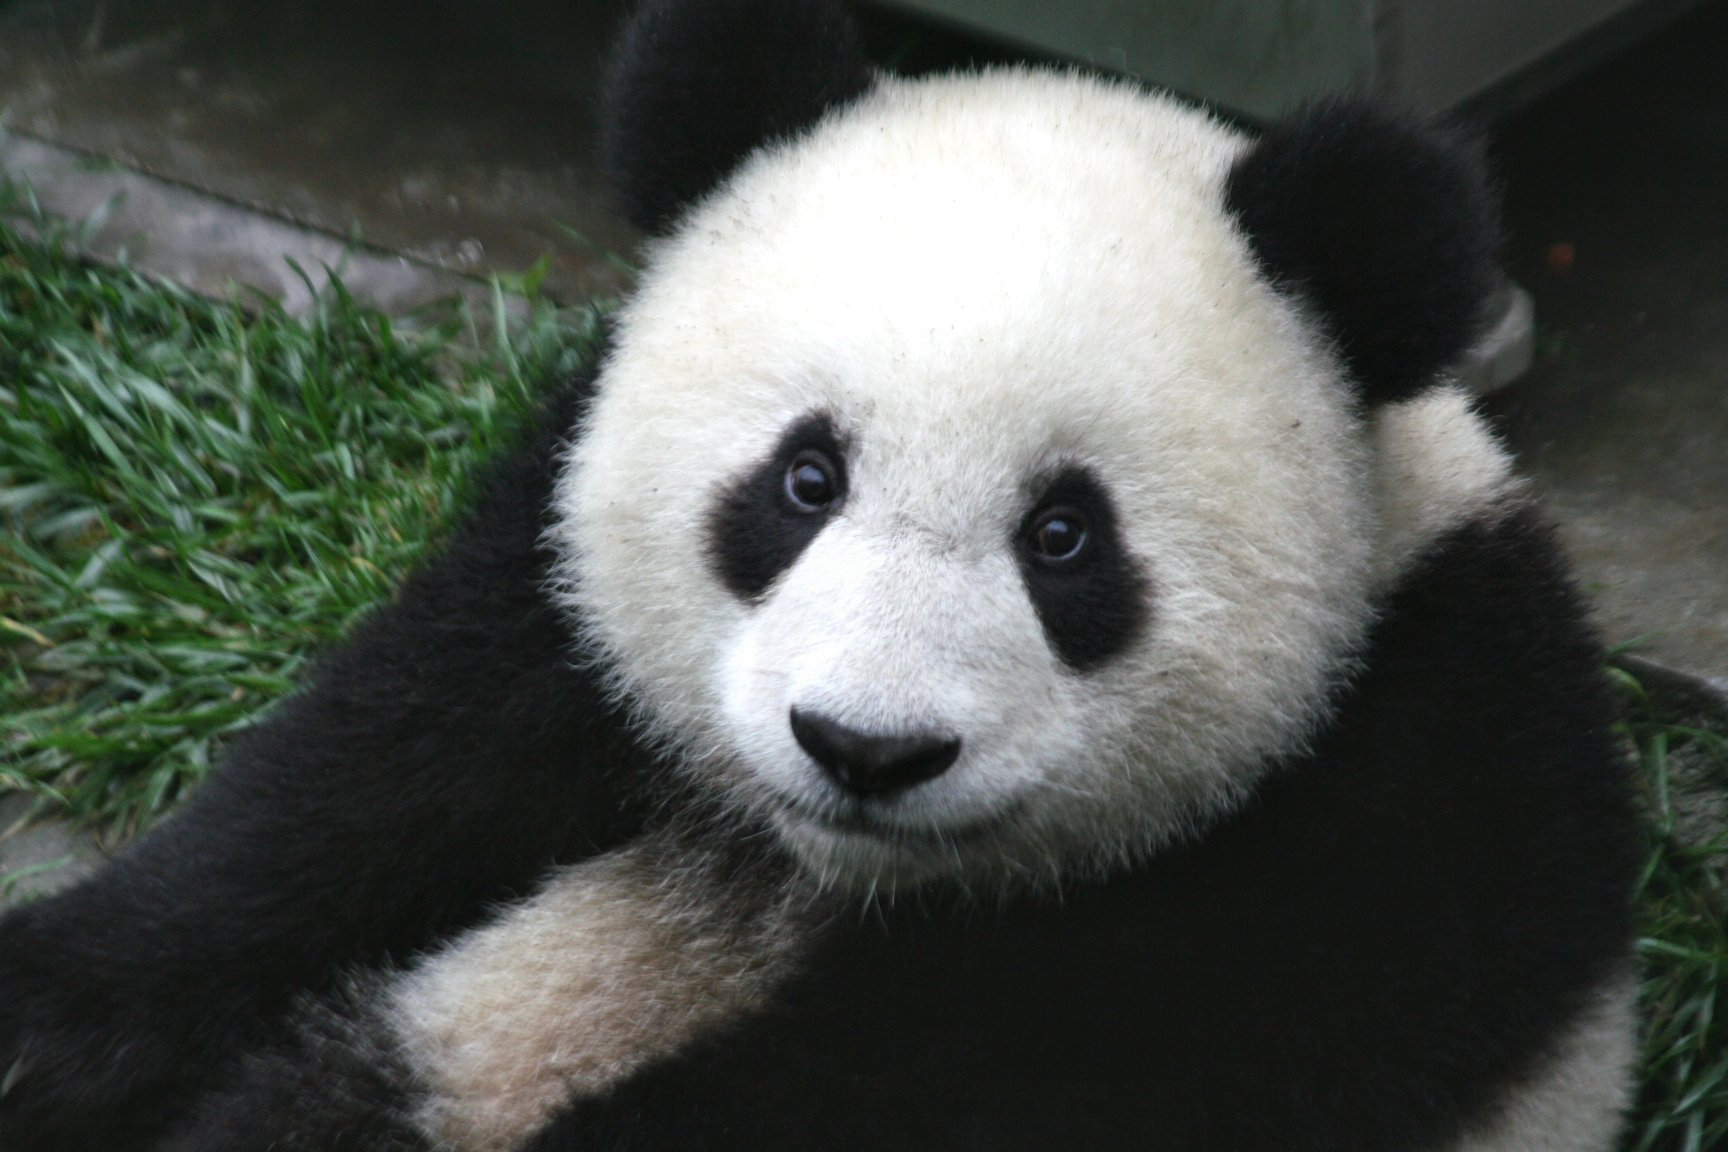
\includegraphics[width=12cm]{figs/pandacub.jpeg}
  \caption{The most adorable animal, hands down.}
  \label{fig:panda}
\end{figure}  

As you know, you can refer back to figure \ref{fig:panda}.

\end{document}

% On Emacs, C-x C-n to evaluate the following before compiling
%%% Local Variables:
%%% LaTeX-command: "latex -shell-escape"
%%% End: